\documentclass[aspectratio=169]{beamer}
\usetheme{Madrid}
\usepackage{booktabs}
\usepackage{graphicx}
\usepackage{array}

\title{Branch Specialization Checkpoint}
\subtitle{Weak Token-Router Supervision Sweep}
\author{Branch Specialization Project}
\date{2026-05-22}

\begin{document}

\begin{frame}
  \titlepage
  \vspace{-0.5em}
  \begin{center}
    Checkpoint reason: gate compliance appears before causal branch modularity.
  \end{center}
\end{frame}

\begin{frame}{Question}
  Previous checkpoint:
  \begin{itemize}
    \item weak token-router supervision at weight 0.05 produced near-oracle
      branch-level functional modularity;
    \item unconstrained learned token routing did not.
  \end{itemize}

  \vspace{0.8em}
  This checkpoint asks:

  \begin{quote}
    How much routing supervision is needed before learned gates become causal
    branch modularity, not just gate preference?
  \end{quote}
\end{frame}

\begin{frame}{Setup}
  Same local-vs-induction competition task and branch model:
  \begin{itemize}
    \item config: \texttt{weak\_token\_router};
    \item local weight 0.25, induction weight 1.0;
    \item five seeds per weight, 1200 training steps;
    \item branch modularity measured by branch ablation, not gate values alone.
  \end{itemize}

  \vspace{0.6em}
  Swept scored-position routing loss weights:
  \begin{center}
    \texttt{0.005, 0.01, 0.02, 0.03, 0.04, 0.045, 0.05}
  \end{center}
\end{frame}

\begin{frame}{Main Evidence}
  \begin{center}
  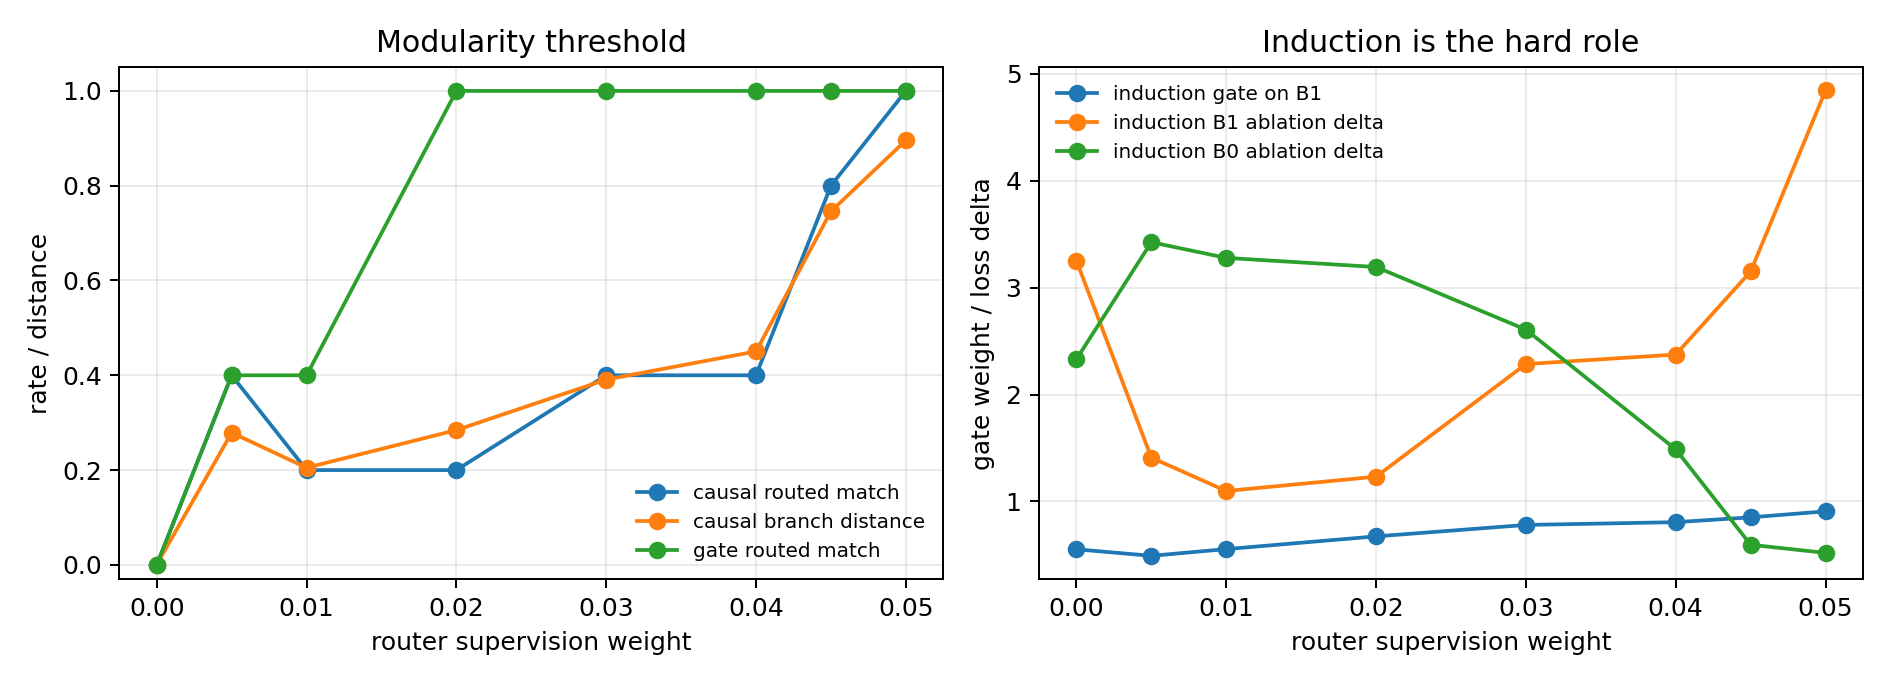
\includegraphics[width=0.92\linewidth]{figures/weak_token_router_sweep.png}
  \end{center}

  \vspace{-0.4em}
  \small
  Gates point the right way before causal ablations become modular. Reliable
  5/5 causal modularity appears only at weight 0.05 in this sweep.
\end{frame}

\begin{frame}{Threshold Table}
  \begin{center}
  \scriptsize
  \begin{tabular}{rrrrrr}
    \toprule
    Weight & Local acc. & Ind. acc. & Gate match & Causal match & Branch dist. \\
    \midrule
    0.000 & 1.0000 & 0.9989 & 0.00 & 0.00 & 0.0006 \\
    0.005 & 1.0000 & 0.9978 & 0.40 & 0.40 & 0.2789 \\
    0.010 & 0.9998 & 0.9987 & 0.40 & 0.20 & 0.2050 \\
    0.020 & 0.9994 & 0.9985 & 1.00 & 0.20 & 0.2844 \\
    0.030 & 0.9999 & 0.9994 & 1.00 & 0.40 & 0.3910 \\
    0.040 & 1.0000 & 0.9983 & 1.00 & 0.40 & 0.4504 \\
    0.045 & 0.9999 & 0.9985 & 1.00 & 0.80 & 0.7459 \\
    0.050 & 0.9998 & 0.9983 & 1.00 & 1.00 & 0.8957 \\
    \bottomrule
  \end{tabular}
  \end{center}

  \vspace{0.5em}
  Causal match means local top branch is 0 and induction top branch is 1 under
  branch ablation.
\end{frame}

\begin{frame}{Per-Seed Pattern}
  \begin{center}
  \scriptsize
  \begin{tabular}{rcc}
    \toprule
    Weight & Local top branches & Induction top branches \\
    \midrule
    0.005 & \texttt{\{0:5\}} & \texttt{\{0:3, 1:2\}} \\
    0.010 & \texttt{\{0:5\}} & \texttt{\{0:4, 1:1\}} \\
    0.020 & \texttt{\{0:5\}} & \texttt{\{0:4, 1:1\}} \\
    0.030 & \texttt{\{0:5\}} & \texttt{\{0:3, 1:2\}} \\
    0.040 & \texttt{\{0:5\}} & \texttt{\{0:3, 1:2\}} \\
    0.045 & \texttt{\{0:5\}} & \texttt{\{0:1, 1:4\}} \\
    0.050 & \texttt{\{0:5\}} & \texttt{\{1:5\}} \\
    \bottomrule
  \end{tabular}
  \end{center}

  \vspace{0.7em}
  Local becomes branch-0-specific at every nonzero weight. Induction is the
  limiting role and flips reliably only near the top of the sweep.
\end{frame}

\begin{frame}{Gate vs Causality}
  \textbf{At weight 0.02:}
  \begin{itemize}
    \item gate routed match = 1.00;
    \item causal routed match = 0.20.
  \end{itemize}

  \vspace{0.6em}
  \textbf{At weight 0.05:}
  \begin{itemize}
    \item gate routed match = 1.00;
    \item causal routed match = 1.00.
  \end{itemize}

  \vspace{0.8em}
  The router can assign positions to the intended branches before the branch
  computations themselves become role-separated.
\end{frame}

\begin{frame}{Interpretation}
  \textbf{Supported in this toy setup:}
  \begin{itemize}
    \item A routing-pressure threshold exists for causal modularity.
    \item Gate metrics alone can overstate functional modularity.
    \item Causal branch ablation is necessary for the modularity claim.
  \end{itemize}

  \vspace{0.6em}
  \textbf{Current threshold estimate:}
  \begin{quote}
    5/5 causal modularity appears at 0.05; 0.045 is near-threshold at 4/5;
    weights at or below 0.04 are mixed.
  \end{quote}
\end{frame}

\begin{frame}{Decision}
  Stop adding labeled-router weights for now.

  \vspace{0.8em}
  Next decisive experiment:
  \begin{quote}
    Test unlabeled routing pressure, such as entropy or load-balancing
    regularization, and ask whether it can produce any similar causal modularity
    shift without role labels.
  \end{quote}

  \vspace{0.8em}
  This distinguishes labeled routing sufficiency from spontaneous or
  regularization-induced modularity.
\end{frame}

\begin{frame}{Sources and Provenance}
  \scriptsize
  \begin{itemize}
    \item Report: \texttt{doc/phase3\_toy\_weak\_router\_sweep.md}
    \item Model script: \texttt{scripts/toy\_branch\_isolation\_intervention.py}
    \item Analysis script: \texttt{scripts/analyze\_weak\_router\_sweep.py}
    \item Sweep output: \texttt{results/phase3\_toy\_weak\_token\_router\_sweep\_analysis/}
    \item Deck data snapshot: \texttt{presentations/2026-05-22-1354-weak-router-sweep/data/}
  \end{itemize}
\end{frame}

\end{document}
